\subsection{The DSLTrans Transformation Language}

% MDD and MTs. Not very important but I do not know how far back should we start.
Model-Driven Development (MDD) is a software engineering approach that uses
models - typically represented as graphs - as first class citizens to create and evolve software systems
\cite{Hailpern:2006vd}.
Model Transformations, prescribed by Model Transformation Languages (MTLs) are the preferred approach to manipulate those models \cite{Software2003}.
MTLs typically describe a set of rules that guide the transformation of models.
Their productivity comes from the fact that those rules can be described elegantly without the accidental complexity of graph manipulation.

% Model translations vs Rewritting Transformations.
Here, a model transformation is defined as a translation, as opposed to a graph rewriting process.
In graph rewriting, a graph representing a model or a set of models gets rewritten continuously according to a set of rules, until some termination criteria is met. 
In a model translation, there is a source model and a target model and the target model is the result of applying the translation to the source model.
Operationally speaking, each of these approaches can mimic the other: graph rewriting can be used to perform model translations (e.g. \cite{Grunske2005}) and model translations, \emph{when applied repetitively}, can perform graph rewriting.

%DSLTrans: why it was used to prove properties.
DSLTrans~\cite{Barroca2011} is an MTL used to specify model translations.
Its main distinctive feature is that the model translations that are described in DSLTrans are guaranteed to always terminate\footnote{This result assumes that finite models are used.}. This feature comes at a cost: DSLTrans is not Turing complete, i.e., no unbounded recursion, non-determinist or element deletion
can be specified. Despite the apparent lack of expressivity, our experience has showed that it is possible to specify a wide range of transformations using DSLTrans. Furthermore, it makes DSLTrans transformations ideal to prove properties about since the set of possible behaviors is finite.

%Why use the families to persons example.
To present the syntax and semantics of DSLTrans, we will be using the Families-to-Persons transformation from the ATL transformation zoo \footnote{\url{http://www.eclipse.org/atl/atlTransformations}}.
Because this transformation can be easily understood, it allows us to focus on the essential concepts of DSLTrans.

%Metamodels of families to persons
Figure~\ref{fig:families_to_persons_metamodels} shows the metamodel of the Family language on the left, and the Community language on the right.
These two languages represent different perspectives of groups of people. A household is composed of one or more families, and each family has a father, mother, daughters and sons.
A community is composed of people and each person can either be a man or a woman.

\begin{figure}
\begin{center}
  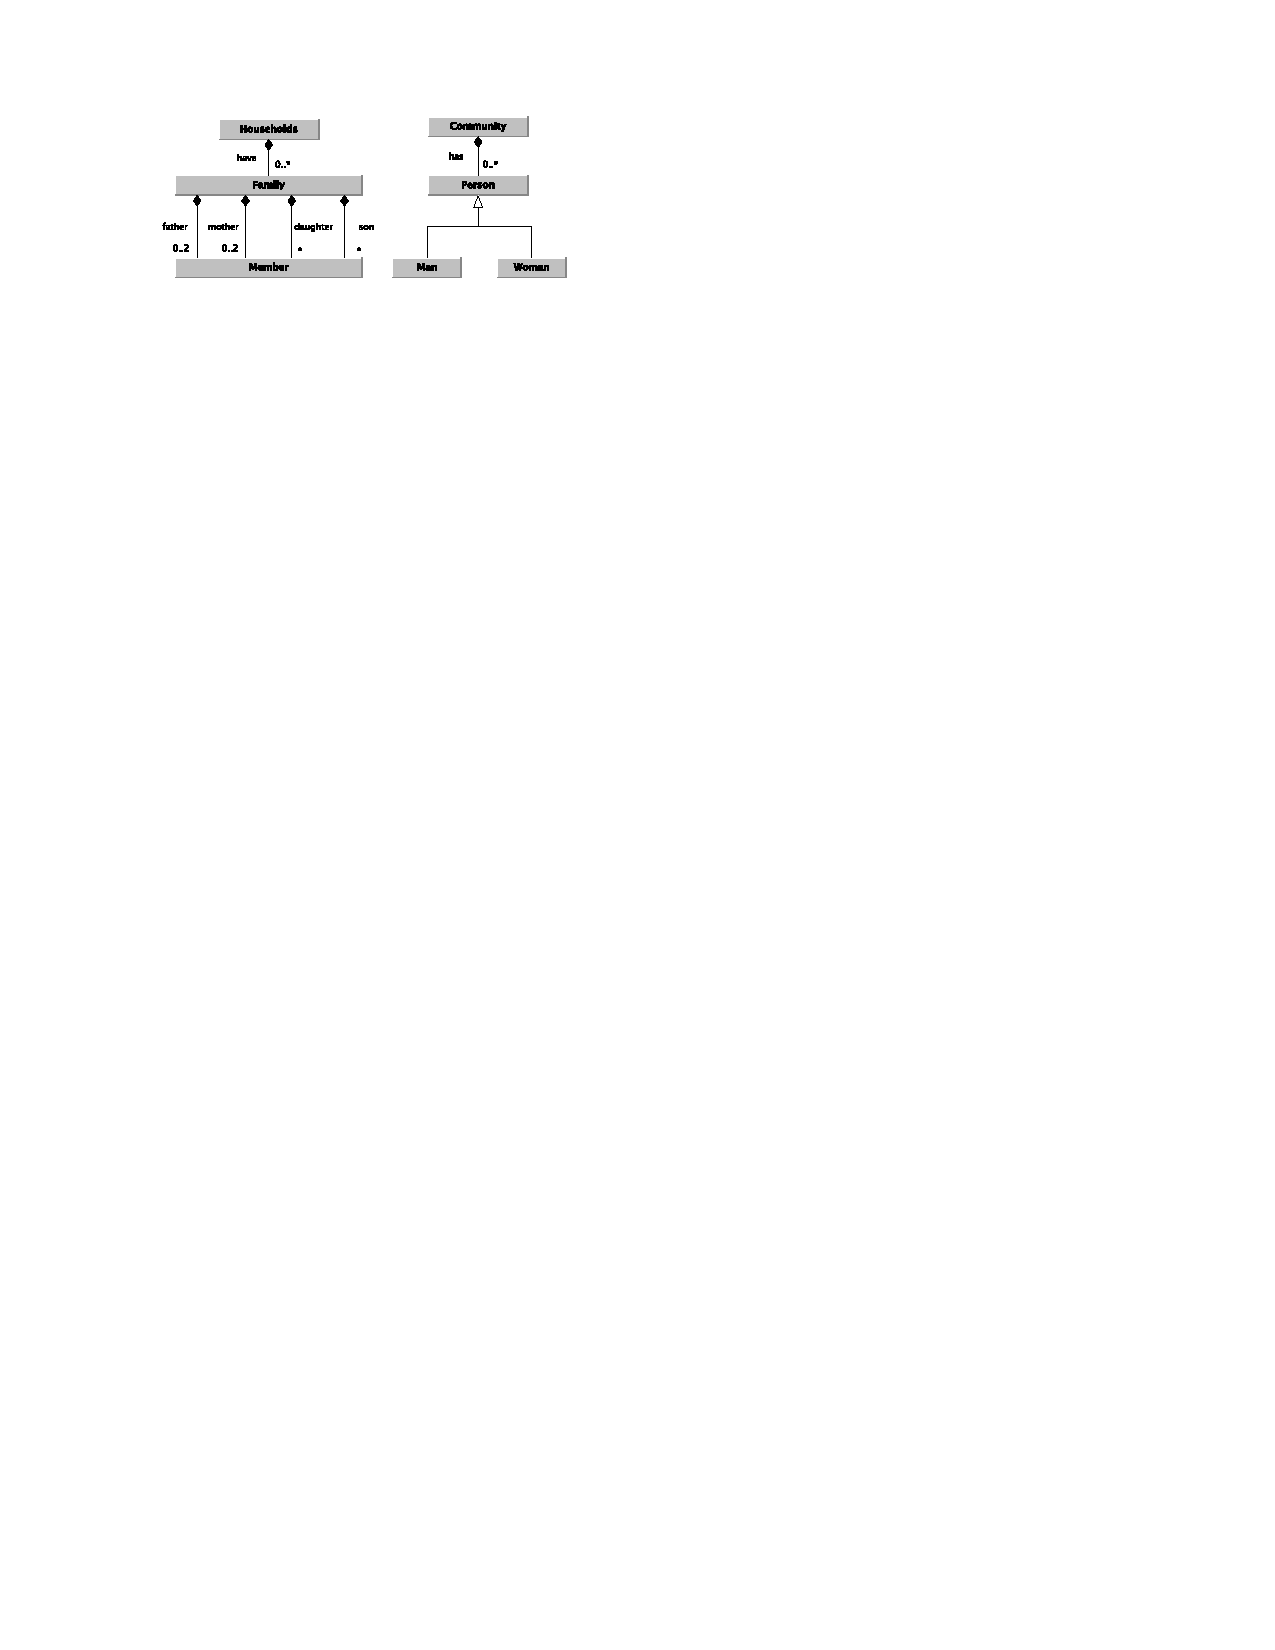
\includegraphics[width=0.5\textwidth]{figures/families_to_persons_metamodels}
  \caption{Families to persons metamodel. Taken from \cite{Oakes}.}
  \label{fig:families_to_persons_metamodels}
\end{center}
\end{figure}

%Informal description of the transformation.
Given a families model, we define a community model by applying the following informal rules:
\begin{asparadesc}
  \item[HouseHold Rule] A household in the families model is translated into a community in the communities model. \cgg{This might change. Need to justify this element. The other rules must be completed depending on how this plays out.}
  \item[Male Member Rule] 
  \item[Female Member Rule]
  \item[Family Member Rule]
\end{asparadesc}

\subsubsection{Syntax}

\subsubsection{Semantics}












